\chapter{Motion Tracking}

In diesem Kapitel möchten wir Ihnen das Motion Tracking näher bringen. Wie der Name ``Motion Tracking'' schon sagt geht es hier um das Folgen einer Bewegungssequenz. Anders als bei den magnetischen und mechanischen Systemen wo die Bewegungen direkt aufgezeichnet werden, müssen bei den optischen Systemen die Bewegungen später am Computer rekonstruiert werden. Diesen Schritt betrachten wir nun ein bisschen genauer.

\section{Absolute Differenz zwischen zwei Bilder}
\label{sec:absolute_diff}
Die einfachste Art um eine Bewegung auf zwei nacheinander folgenden Bilder zu ermitteln ist die Differenz der Bilder zu berechnen. Nehmen wir an wir haben ein Pixel $ u_{t+1}(x,y) $ zum Zeitpunkt $ t+1 $ und das dazugehörige Pixel im vorherigen Bild $ u_{t}(x,y) $. Dann können wir sagen, dass die Subtraktion der Helligkeitswerte der beiden Pixel uns einen Änderungswert ergibt. Weiter können wir eine Minimaländerung im Helligkeitswert definieren (ein Grenzwert $T, $ Threshold). Dieser Grenzwert ist nötig damit die Störsignale (Noise) gefiltert werden können.\\
Statt zwei aufeinander Folgende Bilder zu betrachten wäre es besser wenn auf dem einen Bild nur der Hintergrund ist und auf dem anderen die momentane Aufnahme. Somit könnte man immer auf dem selben Hintergrund Bild den Threshold berechnen und könnte dem Objekt folgen. 

\section{Three-Step Search}
Um Änderungen in zwei Bildern zu finden werden Such-Algorithmen benötigt. Es gibt viele Algorithmen um zwei Einzelbilder zu analysieren. Wir möchten ein solcher Algorithmus genauer betrachten.

\begin{figure}[htbp]
\centering
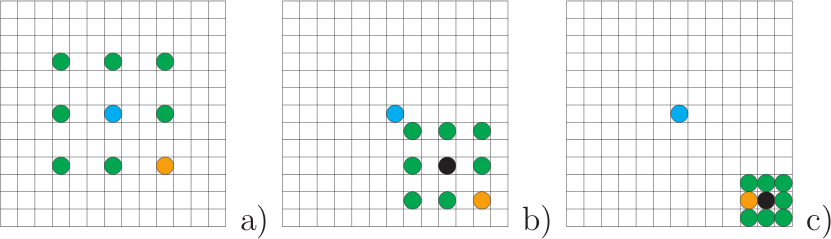
\includegraphics[scale=0.5]{include/3step.png}
\caption{3-Step Search}
\end{figure}

\subsubsection{Algorithmus}
\begin{enumerate}
\item Das Zentrum des Such-Fensters wird als Zentrum für den Algorithmus verwendet. Die Grösse des Such-Fensters definieren wir als $s$. Für die erste Iteration definieren wir die Step-Grösse $p_o = s/2$ und stellen den Iterator  auf $i = 0$ ein.
\item Nächste Step-Grösse wird berechnet $p_{i+1} = p_i/2(gerundet)$
\item Als nächstes werden vom Mittelpunkt aus alle 8 Nachbarn deren absolute Distanz berechnet, welche in einer Distanz von $p_{i+1}$ zum Mittelpunkt entfernt sind.
\item Das beste Ergebnis wird für die nächste Iteration verwendet
\item Falls die Step-Grösse $p{i+1} >1$ überschreitet gehe Zurück zu Schritt 2, ansonsten ist der letzte berechnete Mittelpunkt das beste Ergebnis.
\end{enumerate}

Der Algorithmus ist so optimiert, dass selbst wenn er in drei Schritten noch nicht zum Ziel gelangen konnte, er die Iterationen weiter führt bis zum Ziel. Solche Algorithmen werden Block-Matching Algorithmen genannt, weil sie nicht das ganze Bild analysieren, sondern nur einen gewissen Block um das Ursprungsobjekt. Mit einer Komplexität von $ O(8log_2(s/2))$ kann man sagen, dass dieser Algorithmus recht schnell an ein Ziel führt. Weitere solche Block-matching Algorithmen sind beispielsweise 2d logaritmische Suche, Binäre Suche und Four-Step Suche. Es gibt noch viel mehr, aber grundsätzlich funktionieren die meisten auf die gleiche Art und Weise.
